\documentclass[dvisvgm,tikz,border=4pt]{standalone}
\usepackage{amsmath,amssymb}

\usetikzlibrary{arrows.meta,positioning,automata,shapes,shapes.misc,calc,decorations.pathmorphing,decorations.markings,angles,quotes,patterns,mindmap,matrix,knots,hobby,trees}
\tikzset{->-/.style={decoration={markings, mark=at position 0.5 with {\arrow{Stealth}}}, postaction={decorate}}}
\begin{document}
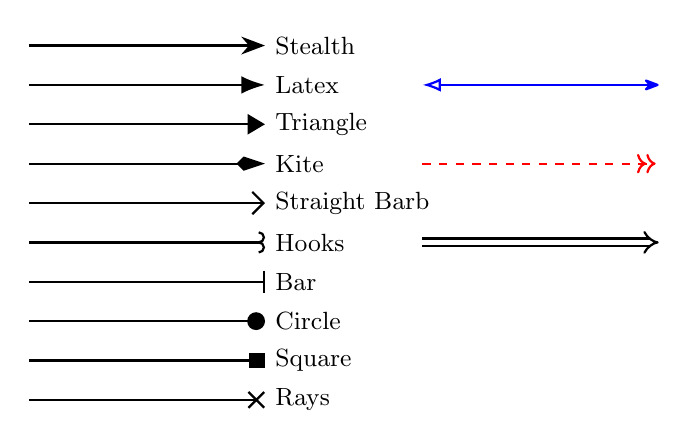
\begin{tikzpicture}[thick]
\foreach \a [count=\i] in {Stealth, Latex, Triangle, Kite, Straight Barb, Hooks, Bar, Circle, Square, Rays}
  \draw[-{\a[scale=1.3]}] (0,-\i*0.5) -- (3,-\i*0.5) node[right, font=\small] {\a};
\draw[{Latex[open]}-{Stealth[round]}, blue] (5,-1) -- (8,-1);
\draw[-{>>[sep]}, red, dashed] (5,-2) -- (8,-2);
\draw[double, -{Implies}, double distance=2pt] (5,-3) -- (8,-3);
\end{tikzpicture}
\end{document}
